\documentclass[11pt,a4paper,twoside]{report}
\usepackage[utf8]{inputenc}
\usepackage[spanish]{babel}
\usepackage{amsmath}
\usepackage{amsfonts}
\usepackage{amssymb}
\author{Nombre y apellidos}

%--------------------------------------------------------
%	Páginas en horizontal
%--------------------------------------------------------

\usepackage{lscape}

%--------------------------------------------------------
%	Hipervínculos de índice
%--------------------------------------------------------

\usepackage{hyperref}

%--------------------------------------------------------
%	Codigo C
%--------------------------------------------------------

\usepackage{listings}

%--------------------------------------------------------
%	Margenes 
%--------------------------------------------------------

\usepackage[margin=3cm]{geometry}

%--------------------------------------------------------
%	Paquetes de graficos y listas
%--------------------------------------------------------

\usepackage{graphicx} % figuras
\usepackage{subfigure} % subfiguras
\usepackage{enumerate} % enumerados

%--------------------------------------------------------
%	Paquetes de imagenes envueltas
%--------------------------------------------------------

\usepackage{wrapfig}

%--------------------------------------------------------
%	encabezados
%--------------------------------------------------------

\usepackage{fancyhdr} 

\lhead[\leftmark]{}
\chead[]{}
\rhead[]{\rightmark}
\renewcommand{\headrulewidth}{0.5pt}

%--------------------------------------------------------
%	pie de pagina
%--------------------------------------------------------

\lfoot[\thepage]{Universidad Politécnica de Madrid}
\cfoot[]{}
\rfoot[Nombre y Apellidos Matricula]{\thepage}
\renewcommand{\footrulewidth}{0.5pt}

%--------------------------------------------------------
%	primera pagina de un capitulo
%--------------------------------------------------------

\fancypagestyle{plain}{
\fancyhead[L]{}
\fancyhead[C]{}
\fancyhead[R]{}
\fancyfoot[L]{}
\fancyfoot[C]{}
\fancyfoot[R]{\thepage}
\renewcommand{\headrulewidth}{0pt}
\renewcommand{\footrulewidth}{0pt}
}

\pagestyle{fancy}

%#########################################################
%	Documento
%#########################################################

\begin{document}

\chapter{}	\label{chap:modelado}

%---------------------------------------------------------
%	1.	Seccion.
%---------------------------------------------------------

\section{}


%\begin{figure}[hb] 
%\centering
%\subfigure[]{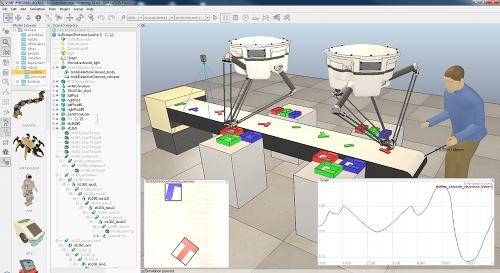
\includegraphics[height=45mm]{../imagenes/3_modelado_rhex/sim_robots_1.png}}
%\subfigure[]{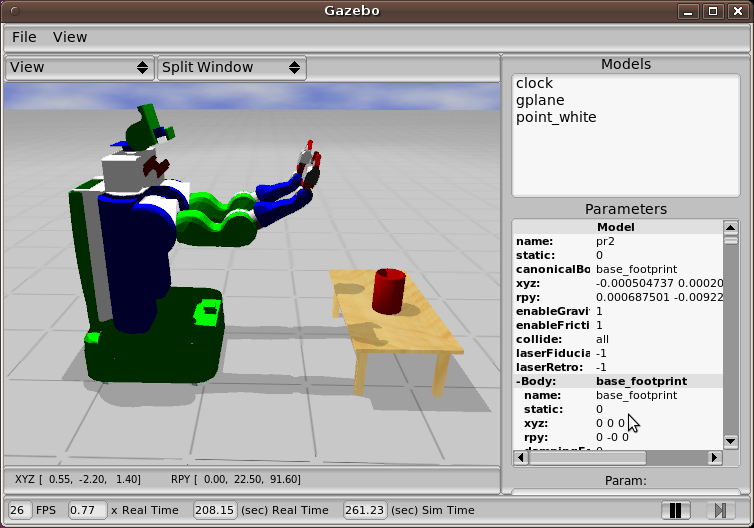
\includegraphics[height=45mm]{../imagenes/3_modelado_rhex/sim_robots_2.png}}
%\caption{Simulaciones de robots en distintos entornos de desarrollo.}
%\end{figure}

% Estilo bibliografia
%\bibliographystyle{acm}
% Archivo bibliografia
%\bibliography{../DB_bibliografia/bib_tfg_raul_cebolla_13069}

\end{document}